% From https://github.com/UWIT-IAM/UWThesis
\documentclass[print]{nuthesis}
\usepackage{amssymb, amsthm, amsmath, amsfonts}
\usepackage{wasysym}
\usepackage{mathrsfs}
% \usepackage{hyperref}
\usepackage{graphicx}
\usepackage{lineno}
\usepackage[colorinlistoftodos]{todonotes}
\usepackage{listings}
%\usepackage{breqn}
\usepackage{cancel, enumerate}
\usepackage{rotating, environ}
\usepackage{caption}
\usepackage{subcaption}
\usepackage[inline]{enumitem}
\usepackage{dirtree}

\newtheorem{thm}{Theorem}
\newtheorem{defn}{Definition}
\newtheorem{prop}{Proposition}
\newtheorem{lemma}{Lemma}
\newtheorem{cor}{Corollary}

% Syntax highlighting #22

%% https://github.com/rstudio/rmarkdown/issues/1649
\newlength{\cslhangindent}
\setlength{\cslhangindent}{1.5em}
\newenvironment{CSLReferences}%
{\setlength{\parindent}{0pt}%
\everypar{\setlength{\hangindent}{\cslhangindent}}\ignorespaces}%
{\par}

% fix for pandoc 1.14
\providecommand{\tightlist}{%
  \setlength{\itemsep}{0pt}\setlength{\parskip}{0pt}}

%% something about tables, from https://github.com/ismayc/thesisdown/issues/122
\usepackage{calc}

%% for copyright symbol
\usepackage{textcomp}

%% to allow to rotate pages to landscape
\usepackage{lscape}
%% to adjust table column width
\usepackage{tabularx}

% suppress bottom page numbers on first page of each chapter
% because they overlap with text
\usepackage{etoolbox}
\patchcmd{\chapter}{plain}{empty}{}{}

%% for more attractive tables
\usepackage{booktabs}
\usepackage{longtable}


\usepackage{graphicx}


% Double spacing, if you want it.
\def\dsp{\def\baselinestretch{2.0}\large\normalsize}
% \dsp

% If the Grad. Division insists that the first paragraph of a section
% be indented (like the others), then include this line:
\usepackage{indentfirst}

%%%%%%%%%%%%%%%%%%
% If you want to use "sections" to partition your thesis
% un-comment the following:
%
% \counterwithout{section}{chapter}
% \setsecnumdepth{subsubsection}
% \def\sectionmark#1{\markboth{#1}{#1}}
% \def\subsectionmark#1{\markboth{#1}{#1}}
% \renewcommand{\thesection}{\arabic{section}}
% \renewcommand{\thesubsection}{\thesection.\arabic{subsection}}
% \makeatletter
% \let\l@subsection\l@section
% \let\l@section\l@chapter
% \makeatother
% 
% \renewcommand{\thetable}{\arabic{table}}
% \renewcommand{\thefigure}{\arabic{figure}}

%%%%%%%%%%%%%%%%%%


%% Stuff from https://github.com/suchow/Dissertate

% The following line would print the thesis in a postscript font

% \usepackage{natbib}
% \def\bibpreamble{\protect\addcontentsline{toc}{chapter}{Bibliography}}

\setcounter{tocdepth}{1} % Print the chapter and sections to the toc
% controls depth of table of contents (toc): 0 = chapter, 1 = section, 2 = subsection

\usepackage{natbib}


% commands and environments needed by pandoc snippets
% extracted from the output of `pandoc -s`
%% Make R markdown code chunks work
\usepackage{array}
\usepackage{amssymb,amsmath}
\usepackage{ifxetex,ifluatex}
\ifxetex
  \usepackage{fontspec,xltxtra,xunicode}
  \defaultfontfeatures{Mapping=tex-text,Scale=MatchLowercase}
\else
  \ifluatex
    \usepackage{fontspec}
    \defaultfontfeatures{Mapping=tex-text,Scale=MatchLowercase}
  \else
    \usepackage[utf8]{inputenc}
  \fi
\fi
\usepackage{color}
\usepackage{fancyvrb}


\ifxetex
  \usepackage[setpagesize=false, % page size defined by xetex
              unicode=false, % unicode breaks when used with xetex
              xetex,
              colorlinks=true,
              linkcolor=blue]{hyperref}
\else
  \usepackage[unicode=true,
              colorlinks=true,
              linkcolor=blue]{hyperref}
\fi
\hypersetup{breaklinks=true, pdfborder={0 0 0}}
\setlength{\parindent}{20pt}
\setlength{\parskip}{6pt plus 2pt minus 1pt}
\setlength{\emergencystretch}{3em}  % prevent overfull lines
\setcounter{secnumdepth}{2} %% controls section numbering, e.g. 1 or 1.2, or 1.2.3



%  ----  Text Colors  ------------------------------------------
%
% Assign colors to writers for review
%
\newcommand{\ear}[1]{{\textcolor{blue}{#1}}}
\newcommand{\svp}[1]{{\textcolor{RedOrange}{#1}}}
\newcommand{\rh}[1]{{\textcolor{Green}{#1}}}
%
\raggedright
\setlength{\parindent}{1cm}

%  --- Code chunk font size -----------------------------------------------
% https://stackoverflow.com/questions/38323331/code-chunk-font-size-in-beamer-with-knitr-and-latexhttps://stackoverflow.com/questions/38323331/code-chunk-font-size-in-beamer-with-knitr-and-latex

%% change fontsize of R code
% \let\oldShaded\Shaded
% \let\endoldShaded\endShaded
% \renewenvironment{Shaded}{\footnotesize\oldShaded}{\endoldShaded}
% 
% %% change fontsize of output
% \let\oldverbatim\verbatim
% \let\endoldverbatim\endverbatim
% \renewenvironment{verbatim}{\footnotesize\oldverbatim}{\endoldverbatim}


\begin{document}
% \linenumbers{}
%% Start formatting the first few special pages
%% frontmatter is needed to set the page numbering correctly
\frontmatter
%% from thesisdown
% To pass between YAML and LaTeX the dollar signs are added by CII
\title{HUMAN PERCEPTION OF EXPONENTIALLY INCREASING DATA DISPLAYED ON A LOG SCALE}
\author{Emily Anna Robinson}
\adviser{Susan VanderPlas and Reka Howard}
\adviserAbstract{}
\major{Statistics}
\degreemonth{August}
\degreeyear{2022}
% \copyrightpage
%%
%% For most people the defaults will be correct, so they are commented
%% out. To manually set these, just uncomment and make the needed
%% changes.
%% \college{Your college}
%% \city{Your City}
%%
%% For most people the following can be changed with a class
%% option. To manually set these, just uncomment the following and
%% make the needed changes.
%% \doctype{Thesis or Dissertation}
%% \degree{Your degree}
%% \degreeabbreviation{Your degree abbr.}
%%
%% Now that we know everything we need, we can generate the title page
%% itself.
%%
\maketitle


\begin{abstract}
    Log scales are often used to display data over several orders of magnitude within one graph. During the COVID-19 pandemic, we have seen both the benefits and the pitfalls of using log scales to display case counts. Three graphical experimental tasks were conducted to evaluate the impact our choice of scale has on human perception of exponentially increasing trends. The first experiment evaluates whether our ability to perceptually notice differences in exponentially increasing trends is impacted by the choice of scale. We conducted a visual inference experiment in which participants were shown a series of lineup plots (consisting of 19 null panels and 1 target panel) and asked to identify the panel that was most different from the others. Our results indicated that when there was a large difference in curvature between the target plot and null plots, the choice of scale had no impact and participants accurately differentiated between the two curves on both the linear and log scale. However, displaying exponentially increasing data on a log scale improved the accuracy of differentiating between models with slight curvature differences. An exception occurred when identifying a plot with curvature embedded in surrounding plots closely relating to a linear trend, indicating that it is easy to identify a curve in a group of lines but much harder to identify a line in a group of curves. The use of visual inference to identify these guidelines suggests that there are \emph{perceptual} advantages to log scales when differences are subtle. Our other experimental tasks focus on determining whether there are cognitive disadvantages to log scales: do log scales make it harder to make use of graphical information? We conducted a graphical task similar to the New York Times ``You Draw It'' page to test an individual's ability to use and make predictions for exponentially increasing data. We asked participants to draw a line using their computer mouse through the increasing exponential trend shown on both scales. In addition to differentiation and prediction of exponentially increasing data, we conduct an experimental task to test an individuals' ability to translate a graph of exponentially increasing data into real value quantities and extend their estimations by making comparisons. The results of our experimental tasks allow us to provide guidelines for readers to actively choose which of many possible graphics to draw, according to some set of design choices, to ensure that our charts are effective. \emph{(399 words; 350 word limit)}
\end{abstract}

%% Optional
%% \begin{copyrightpage}
%% \end{copyrightpage}

%% Optional
% \begin{dedication}
% Dedicated to\ldots{}
% \end{dedication}

%%%%%%%%%%%%%%%%%%%
% Acknowledgments
%%%%%%%%%%%%%%%%%%%
\begin{acknowledgments}
Thank you to all my people!
\end{acknowledgments}
%%%%%%%%%%%%%%%%%%%

%%%%%%%%%%%%%%%%%%%
% Grant Information
%%%%%%%%%%%%%%%%%%%
% \begin{grantinfo}
%     % Add any grant info here
% \end{grantinfo}

%%%%%%%%%%%%%%%%%%%
% ToC
%%%%%%%%%%%%%%%%%%%
\tableofcontents

%%%%%%%%%%%%%%%%%%%
% List of Figures
%%%%%%%%%%%%%%%%%%%
\listoffigures
\listoftables

%%%%%%%%%%%%%%%%%%%
% Start of the document
%%%%%%%%%%%%%%%%%%%
\mainmatter


\hypertarget{literature-review}{%
\chapter{Literature Review}\label{literature-review}}

Editing text colors: \ear{Emily's editing color.} Emily may also use mostly black text as well. \svp{Susan's editing color.} \rh{Reka's editing color.}

\hypertarget{introduction-to-graphics}{%
\section{Introduction to Graphics}\label{introduction-to-graphics}}

Advanced technology and computing power has promoted data visualization as a central tool in modern data science (Unwin, 2020).
Data visualization is defined as the art of drawing graphical charts in order to display data.
Vanderplas, Cook, \& Hofmann (2020) describe the process of creating a graphic from a dataset through the use of variable mapping, data transformations, coordinate systems, and aesthetic features.
Graphics are useful for data cleaning, exploring data structure, and have been an essential component in communicating information for the last 200 years (Lewandowsky \& Spence, 1989; Unwin, 2020; Vanderplas, Cook, \& Hofmann, 2020)
During the 20th century, companies began utilizing graphics to understand their mechanics and support business decisions; news sources began displaying graphics of weather forecasts as a means to communicate critical information and aid in decision-making (Vanderplas, Cook, \& Hofmann, 2020).
Today, we encounter data visualizations everywhere, researchers include graphics to communicate their results in scientific publications and mass media relies on graphics to convey news stories to the public through newspapers, TV, and the Web (Unwin, 2020).

In general, the public holds the self perception that numbers are difficult to understand and that they did not perform well in mathematics during school (Unwin, 2020).
In contrary, there tends to be a positive self perception when it comes to graphics as they are viewed more as illustrations and not as critical parts of an argument (Unwin, 2020).
While tables can be burdensome to readers, graphics can improve the interpretation and representation of the same data (Uri \& Haemer, 1948).
Shah, Mayer, \& Hegarty (n.d.) presents an opposing argument claiming there are still difficulties interpreting and explaining quantitative information depicted in graphs.
One explanation for the opposing views is that the general public is untrained in the ability required in the evaluation of graphic material.
The complexity of graphic devices is directly related to the degree and formality of training necessary for understanding (Haemer \& Kelley, 1949).

Although statistical graphics have become widely used and valued in science, business, and in many other aspects of life, as creators of graphics, we are too accepting of them as default without asking critical questions about the graphics we create or view (Unwin, 2020).
Vanderplas, Cook, \& Hofmann (2020) poses the general question we must ask ourselves, ``how effective is this graph at communicating useful information?''
Higher quality of technology has influenced the creation, replication, and complexity of graphics as there are an infinitely many number of graphical displays and design choices that can be implemented at faster speeds with more flexibility.
The creator of a graphic makes decisions about the variables displayed, the type of graphic, the size of the graphic and the aspect ratio, the colors and symbols used, the scales and limits, the ordering of categorical variables, and the ordering of variables in multivariate displays (Unwin, 2020).
In response to the increasing number of design choices, consistent themes and higher standards are being placed on graphics.
Selecting from an extensive styles and choices of graphics in order effectively communicate insights into the data is a challenging task (Unwin, 2020).
A consistent concern is the lack of theory of graphics available to build on; better theory should result in better graphics (Unwin, 2020).
Creators of graphics need an established set of concepts and terminology to build their graphics from so they can actively choose which of many possible graphics to draw to ensure their charts are effective (Unwin, 2020).

Many efforts have been made to provide guidelines for graphical designs including Wilkinson's Grammar of Graphics \ear{CITE}.
These guidelines provide the ground work necessary for data plots to be depicted and interpreted as statistics (Majumder, Hofmann, \& Cook, 2013).
Vanderplas, Cook, \& Hofmann (2020) define a statistic as, ``a functional mapping of a variable or set of variables.''
The grammar of graphics constructs visual statistics through the use of ``tidy data,'' charactarized as a data set in which each variable is in its own column, each observation is in its own row, and each value is in its own cell (Wickham \& Grolemund, 2016).
The grammar allows variables, as designated in columns, to be mapped to different elements of the graphic such as the axes, colors, shapes, or facets.
Software, such as Hadley Wickham's ggplot2 \ear{CITE}, aims to implement these guidelines recommended through the grammar of graphics.\\
Later, it is illustrated how the structure of ``tidy data'' and the construction of graphics as statistics aid themselves for easy experimentation which allows researchers to compare the effectiveness and understand the perception of different types of charts Vanderplas, Cook, \& Hofmann (2020).
It is important to consider the purpose and motivation behind the generation of the chart as well as the complexity and intended audience you intend to view the chart (Vanderplas, Cook, \& Hofmann, 2020).
A general guideline when generating graphics is to keep it familiar in order to not intimidate and to encourage further interaction from our readers (Unwin, 2020).
Despite past attempts to improve the use of graphics in science, Gordon \& Finch (2015) evaluated 97 graphs for overall quality, based on five principles of graphical excellence, and found there is still an astonishing lack in the quality of graphics. More startling is the fact that the source of the graphic from an applied science or a statistics graphic had no effect on the quality of the graphic (Gordon \& Finch, 2015).
The improvement in graphics depends on both a better definition of variables, units of measurements, scales, and other graphical elements as well as a typical use of grid lines on an accepted set of graphical forms (Gordon \& Finch, 2015).
with the support of changes in software defaults, future work must be done in order to implement the academic research being conducted in graphics into practice for both academics and non-academics in order to achieve a higher standard of the graphics being presented (Vanderplas, Cook, \& Hofmann, 2020).

\hypertarget{graphical-experiments}{%
\section{Graphical Experiments}\label{graphical-experiments}}

In order to provide a set of principles to guide design choices, we must evaluate these design choices through
the use of graphical tests. These tests may take many forms: identifying differences in graphs, reading information
off of a chart accurately, using data to make correct real-world decisions, or predicting the next few observations.
All of these types of tests require different levels of use and manipulation of the information presented in the chart.
The initial push to develop classification and recommendation systems for charts was grounded on heuristics rather than on experimentation (Vanderplas, Cook, \& Hofmann, 2020).
Request were made for the validation of the perception and utility of statistical charts through graphical experiments.
Initial experiments struggled with methodological issues \ear{[CITE: Eells (1926), Croxton and Stryker (1927) and Croxton (1932)]} with most early experimentation stemmed from pyschophysics research on the perception of size and shape \ear{[CITE: Teghtsoonian (1965)]}; these early experiments depended on speed and accuracy for plot evaluation.
Cognitive psychologists and statisticians made progress by conducting experiments to identify perceptual errors associated with different styles of graphics and charts {[}\ear{CITE: Spence 1990}; Cleveland \& McGill (1985){]}.
These later experiments relied on similar methodology as early studies by relying on participants directly reading information from the charts to provide a quantitative estimate or answering a predefined question; as with the early studies, accuracy and response time being evaluated (Peterson and Schramm 1954, Cleveland \& McGill (1984), Broersma and Molenaar 1985, Dunn 1988, Tan 1994, Amer 2005).
Cleveland \& McGill (1984) provide a basis for perceptual judgment, still utilized today, by examining six basic stimuli: position along a common scale, position along nonaligned scales, length, angle, slope, and area.
Other experiments established the notion that redesigning graphs can result in the improvement of the viewer's interpretation (Shah, Mayer, \& Hegarty, n.d.). This is done by relying on gestalt principles to minimize the inferential processes and maximize the pattern association processes required to interpret relevant information. The viewer must first encode the visual array by identifying meaningful visual features, such as a straight light slanting downward. Next, the viewer must classify the quantitative measures and relationships in which those visual features illustrate, such as a decreasing linear relationship between x and y.
The last step involves translating the quantiative measures and relationships to the variables defined in the data set, such as a population decreasing over years.
These studies establish the process in which viewers interact with charts by first perceptually observing the visual features and later translating to cognitive processing of the information depicted by those features \ear{[CITE: Carpenter and Shah, 1998]}.
In recent years, there have been advancements in the methodology used to investigate the effectiveness of statistical charts (Vanderplas, Cook, \& Hofmann, 2020). Some of the new methods, such as the lineup protocol (Buja et al., 2009), utilize the grammar of graphics designation of a data plot as a statistic through the functional mapping of variable(s). This allows the data plot to be tested similar to other statistics, by comparing the actual data plot to a set of plots with the absence of any data structure we can test the likelihood of any perceived structure being significant (Vanderplas, Cook, \& Hofmann, 2020).
While the methodology of these recent experiments differs from earlier studies, the focus is still placed on the initial perception and graph comprehension with a relatively small amount of work conducted to understand the effect of design choices on higher cognitive processes such as learning or analysis \ear{[CITE: Green and Fisher 2011]}.
Most recent graphics experiments have utilized tools such as Amazon Turk, Prolific, Reddit, and other crowd sourcing websites to evaluate the psychophysics and patterns associated with design choices (VanderPlas \& Hofmann, 2017).

\hypertarget{logarithmic-scales-and-mapping}{%
\section{Logarithmic Scales and Mapping}\label{logarithmic-scales-and-mapping}}

Logarithms convert multiplicative relationships to additive ones, providing an elegant way to span many orders of magnitude, to show elasticities and other proportional changes, and to linearize power laws.
They also have practical purposes, easing the computation of small numbers such as likelihoods and transforming data to fit statistical assumptions.
When faced with data which spans several orders of magnitude, we must decide whether to show the data on its original scale (compressing the smaller magnitudes into relatively little area) or to transform the scale and alter the contextual appearance of the data.
One common solution is to use a log scale transformation to display data over several orders of magnitude within one graph. Logarithms make multiplicative relationships additive, showing elasticities and other proportional changes, and also linearize power laws Menge et al. (2018)
When presenting log scaled data, it is possible to use either un-transformed scale labels (for example, values of 1, 10 and 100 are equally spaced along the axis) or log transformed scale labels (for example, 0, 1, and 2, showing the corresponding powers of 10).

\begin{itemize}
\item
  At the beginning of the SARSNCOV-2 pandemic (COVID-19), we saw an influx of dashboards being developed to display case counts, transmission rates, and outbreak regions GmbH (2020); mass media routinely showed charts to share information with the public about the progression of the pandemic Romano, Sotis, Dominioni, \& Guidi (2020). People began seeking out graphical displays of COVID-19 data as a direct result of these pieces of work GmbH (2020); providing increased and ongoing exposure to these graphics over time. Many of these graphics helped guide decision makers to implement policies such as shut-downs or mandated mask wearing, as well as facilitated communication with the public to increase compliance Bavel et al. (2020).
\item
  We have recently experienced the benefits and pitfalls of using log scales as COVID-19 dashboards displayed
  case count data on both the log and linear scale {``An interactive visualization of {COVID}-19 {{}} 91-{DIVOC}''} (n.d.) {``Coronavirus chart''} (n.d.). In spring 2020, during the early stages of the COVID-19 pandemic, there were large magnitude discrepancies in case counts at a given time point between different geographic regions (e.g.~states and provinces as well as countries and continents). During this time, we saw the usefulness of log scale transformations showing case count curves for areas with few cases and areas with many cases within one chart. As the pandemic evolved, and the case counts were no longer spreading exponentially, graphs with linear scales seemed more effective at spotting early increases in case counts that signaled more localized outbreaks.
\item
  This is only one recent example of a situation in which both log and linear scales are useful for showing different aspects of the same data; there are long histories of using log scales to display results in ecology, psychophysics, engineering, and physics {``Log {Scale}''} (n.d.) Menge et al. (2018) Heckler, Mikula, \& Rosenblatt (2013)
\item
  The necessary training required in the appraisal of graphic material may be more involved, for example when an ordinate must be associated with the logarithm of a magnitude. Haemer \& Kelley (1949)
  Overall, these results reveal both universal and culture-dependent facets of the sense of number. After a minimal instruction period, even members of a remote culture with reduced vocabulary and education readily understand that number can be mapped onto a spatial scale. The exact form of this mapping switches dramatically from logarithmic to linear, however, depending on the ages at which people are tested, the education they have received, and the format in which numbers are presented. {``Log or {Linear}? {Distinct} {Intuitions} of the {Number} {Scale} in {Western} and {Amazonian} {Indigene} {Cultures}''} (n.d.)
\item
  In American children, logarithmic mapping does not disappear all at once, but vanishes first for small numbers and much later for larger numbers from 1 to 1000 (up to fourth or sixth grade in some children). {``Log or {Linear}? {Distinct} {Intuitions} of the {Number} {Scale} in {Western} and {Amazonian} {Indigene} {Cultures}''} (n.d.)
\item
  Whole number magnitude representations progress from a compressive, approximately logarithmic distribution to an approximately linear one. Transitions occur earlier for smaller than for larger ranges of whole numbers, corresponding both to the complexity of the numbers and to the ages when children gain experience with them. Estimation proceeds logarithmically initially and transitions to linear later in development, for several different numerical ranges. Siegler \& Braithwaite (2017)
\item
  Certain graphic forms are inseparable from concepts that require special training for their understanding and in such cases the relative difficulty is intrinsic. Curves plotted on double logarithmic paper on on probability paper are typical examples of this type. Semi - Logarithmic chart for Temporal series falls under the ``understanding calls for a certain degree of technical training'' Haemer \& Kelley (1949)
\item
  Therefore, if a continuumbetween perceptual and cognitive processes exists, numerical representations should also be represented on a nonlinear, compressed ``number scale.'' Nieder \& Miller (n.d.)
\item
  the idea is that compression enlarges the coding space, thus increasing the dynamic range of perception and firing neurons. Nieder \& Miller (n.d.)
\end{itemize}

Our inability to accurately predict exponential growth might also be addressed by log transforming the data, however, this transformation introduces new complexities; most readers are not mathematically sophisticated enough to intuitively understand logarithmic math and translate that back into real-world effects.
In Menge et al. (2018), ecologists were surveyed to determine how often ecologists encounter log scaled data and how well ecologists understand log scaled data when they see it in the literature.
Participants were presented two relationships displayed on linear-linear scales, log-log scales with untransformed values, or log--log scales with log transformed values.
Menge et al. (2018) propose three types of misconceptions participants encountered when presented data on log-log scales: `hand-hold fallacy,' `Zeno's zero fallacy,' and `watch out for curves fallacies.' These misconceptions are a result of linear extrapolation assuming that a line in log-log space represents a line instead of the power law in linear-linear space. The study found that in each of these scenarios, participants were confident in their incorrect responses, indicating incorrect knowledge rather than a lack of knowledge. The `hand-hold falacy' stems from the misconception that steeper slopes in log-log relationships are steeper slopes in linear-linear space. In fact, it is not only the slope that matters, but also the intercept and the location on the horizontal axis since a line in log-log space represents a power law in linear-linear space (i.e.~linear extraploation). Emerging from `Zeno's zero fallacy' is the misconception that positively sloped lines in log-log space can imply a non-zero value of y when x is zero. This is never true as positively sloped lines in log-log space actually imply that y = 0 when x = 0. This misconception again is a result of linear extrapolation assuming that a line in log-log space represents a line instead of the power law in linear-linear space. The last misconception, `watch out for curves fallacies' encompasses three faults: (1) lines in log-log space are lines in linear-linear space, (2) lines in log-log space curve upward in linear-linear space, and (3) curves in log-log space have the same curvature in linear-linear space. Linear extrapolation is again responsible for the first and third faults while the second fault is a result of error in thinking that log-log lines represent power laws (which are exponential relationships), and all exponential relationships curve upward; this is only true when the log-log slope is greater than 1. Menge et al. (2018) found that in each of these scenarios, participants were confident in their incorrect responses, indicating incorrect knowledge rather than a lack of knowledge.

\hypertarget{psychophysics}{%
\section{Psychophysics}\label{psychophysics}}

\begin{itemize}
\item
  ``Preattentive perceptual effects are those which do not require sustained cognitive attention; they are processed automatically within the first 500 milliseconds of viewing a chart or graph. Components processed preattentively include colour and shape, as well as some basic information about coarse relationships between individual components.'' Vanderplas, Cook, \& Hofmann (2020)
\item
  Preattentively processed features include shape, angle, size, and texture; however, typically, combinations of preattentive features which represent separate features in the data are processed attentively
  After the preattentive stage, attention is necessary for subsequent processing; this directed attention scaffolds relationships between components and helps us interpret the chart or graph in context. Most of the insights we gain from charts and graphs are due to the cognitive processes that occur after attention is focused on specific aspects of the graph. Vanderplas, Cook, \& Hofmann (2020)
\item
  According to a cognitive analysis, graph interpretation involves (a) relatively simple pattern perception and association processes in which viewers can associate graphic patterns to quantitative referents and (b) more complex and error-prone inferential processes in which viewers must mentally transform data. Shah, Mayer, \& Hegarty (n.d.)
\item
  There are limits to what one can test using direct estimation: it is generally preferable to test only very straightforward assessments of the content of a chart or graph, to fit within a simple experimental paradigm. Some studies of graphs utilize psychophysics methodology to assess data visualizations. Initially, of course, a significant portion of the research in statistical graphics came from the fields of psychophysics and cognitive psychology (Spence 1990, Teghtsoonian 1965, Lewandowsky and Spence 1989), but in most cases this was not accompanied by a use of the methods of psychophysics for experimental texting of charts and graphcs. Psychophysical experimental design is focused on whether an effect is detectable, and whether the magnitude of the effect can be accurately estimated. Psychophysics and direct
  observation studies are limited by the questions that are asked; Vanderplas, Cook, \& Hofmann (2020)
\item
  Other methods: Thinking aloud, Eye Tracking, etc. Vanderplas, Cook, \& Hofmann (2020)
\item
  \textbf{Webers Law}

  \begin{itemize}
  \tightlist
  \item
    Weber's law: the fact that larger numbers require a proportional larger difference in order to remain equally discriminate. {``Log or {Linear}? {Distinct} {Intuitions} of the {Number} {Scale} in {Western} and {Amazonian} {Indigene} {Cultures}''} (n.d.)
  \item
    we do not notice absolute changes in stimuli; we notice relative changes. Sun, Wang, Goyal, \& Varshney (2012)
  \item
    Weber--Fechner law. It states that perceived intensity P is logarithmic to the stimulus intensity S (above a minimal threshold of perception S0) Sun, Wang, Goyal, \& Varshney (2012)
  \end{itemize}
\item
  \textbf{Underestimation of Exponential Growth}

  \begin{itemize}
  \tightlist
  \item
    In fact, early studies explored the estimation and prediction of exponential growth, finding that growth is underestimated when presented both numerically and graphically but that numerical estimation is more accurate than graphical estimation for exponential curves Wagenaar \& Sagaria (1975). One way to improve estimation of increasing exponential trends is to provide immediate feedback to participants about the accuracy of their current predictions Mackinnon \& Wearing (1991). While prior contextual knowledge or experience with exponential growth does not improve estimation, instruction on exponential growth reduces the underestimation: participants adjust their initial starting value but not their perception of growth rate Wagenaar \& Sagaria (1975), Jones (1977).
  \end{itemize}
\item
  \textbf{Risk Assessment}
\end{itemize}

\hypertarget{visual-inference}{%
\section{Visual Inference}\label{visual-inference}}

To lay a foundation for future exploration of the use of log scales, we begin with the most fundamental ability to identify differences in charts; this does not require that participants understand exponential growth, identify log scales, or have any mathematical training. Instead, we are simply testing the change in perceptual sensitivity resulting from visualization choices.

A statistic is a numerical function which summarizes the data; by this definition, graphs are visual statistics.
To evaluate a graph, we have to run our statistic through a visual evaluation - a person. If two different methods
of presenting data result in qualitatively different results when evaluated visually, then we can conclude that the visual statistics are signiffcantly different. Recent graphical experiments have utilized statistical lineups to quantify the perception of graphical design choices{[}VanderPlas and Hofmann, 2017, Hofmann et al., 2012, Loy et al., 2016{]}. Statistical lineups provide an elegant way of combining perception and statistical hypothesis testing using graphical experiments {[}Wickham et al., 2010, Majumder et al., 2013, Vanderplas et al., 2020b{]}. `Lineups' are named after the `police lineup' of criminal investigations where witnesses are asked to identify the criminal from a set of
individuals. Similarly, a statistical lineup is a plot consisting of smaller panels; the viewer is asked to identify the plot of the real data from among a set of decoy null plots. A statistical lineup typically consists of 20 panels - 1 target panel and 19 null panels (Figure 1). If the viewer can identify the target panel embedded within the set of null panels, this suggests that the real data is visually distinct from data generated under the null model. Crowd sourcing websites such as Amazon Mechanical Turk, Reddit, and Prolifc allow us to collect responses from multiple
viewers. In this paper, we use statistical lineups to test our ability to differentiate between exponentially increasing curves with differing levels of curvature, using linear and log scales.

\begin{itemize}
\tightlist
\item
  Explicit graphical tests, as we have referred to them, are tests where the user is directed to assess a specific feature of a plot or answer a specific question. Vanderplas, Cook, \& Hofmann (2020)
  implicit graphical test, the user must identify both the purpose and function of the plot and use that information to evaluate the plots as shown. Visual inference (pg 14) problems. Vanderplas, Cook, \& Hofmann (2020)
  Implicit graphical tests approach the problem of spurious plot relationships at the level of the data, leveraging the human visual system to conduct a suite of visual tests for features such as outliers, clusters, linear and nonlinear relationships. The advantage to implicit testing is that lineups do not require a specification of a feature of interest in the testing framework, Vanderplas, Cook, \& Hofmann (2020)
\end{itemize}

\hypertarget{you-draw-it}{%
\section{You Draw It}\label{you-draw-it}}

\begin{itemize}
\tightlist
\item
  advocate smoothing of scatterplots to assist in detecting the shape of the point cloud in situations where the error in the data is substantial, or where the density of points changes along the abscissa Cleveland \& McGill (1984)
\end{itemize}

\hypertarget{graphics-context-questions}{%
\section{Graphics Context Questions}\label{graphics-context-questions}}

\begin{itemize}
\tightlist
\item
  Such complex inferential processes involve quantitatively transforming the information in the display (e.g., mentally transforming from a linear to logarithmic scale or calculating the difference between two or more data points; Cleveland, 1984, 1985).
\end{itemize}

\hypertarget{lineups}{%
\chapter{Perception through lineups}\label{lineups}}

\hypertarget{introduction}{%
\section{Introduction}\label{introduction}}

To lay a foundation for future exploration of the use of log scales, we begin with the most fundamental ability to identify differences in charts; this does not require that participants understand exponential growth, identify log scales, or have any mathematical training.
Instead, we are simply testing the change in perceptual sensitivity resulting from visualization choices.

\begin{figure}

{\centering 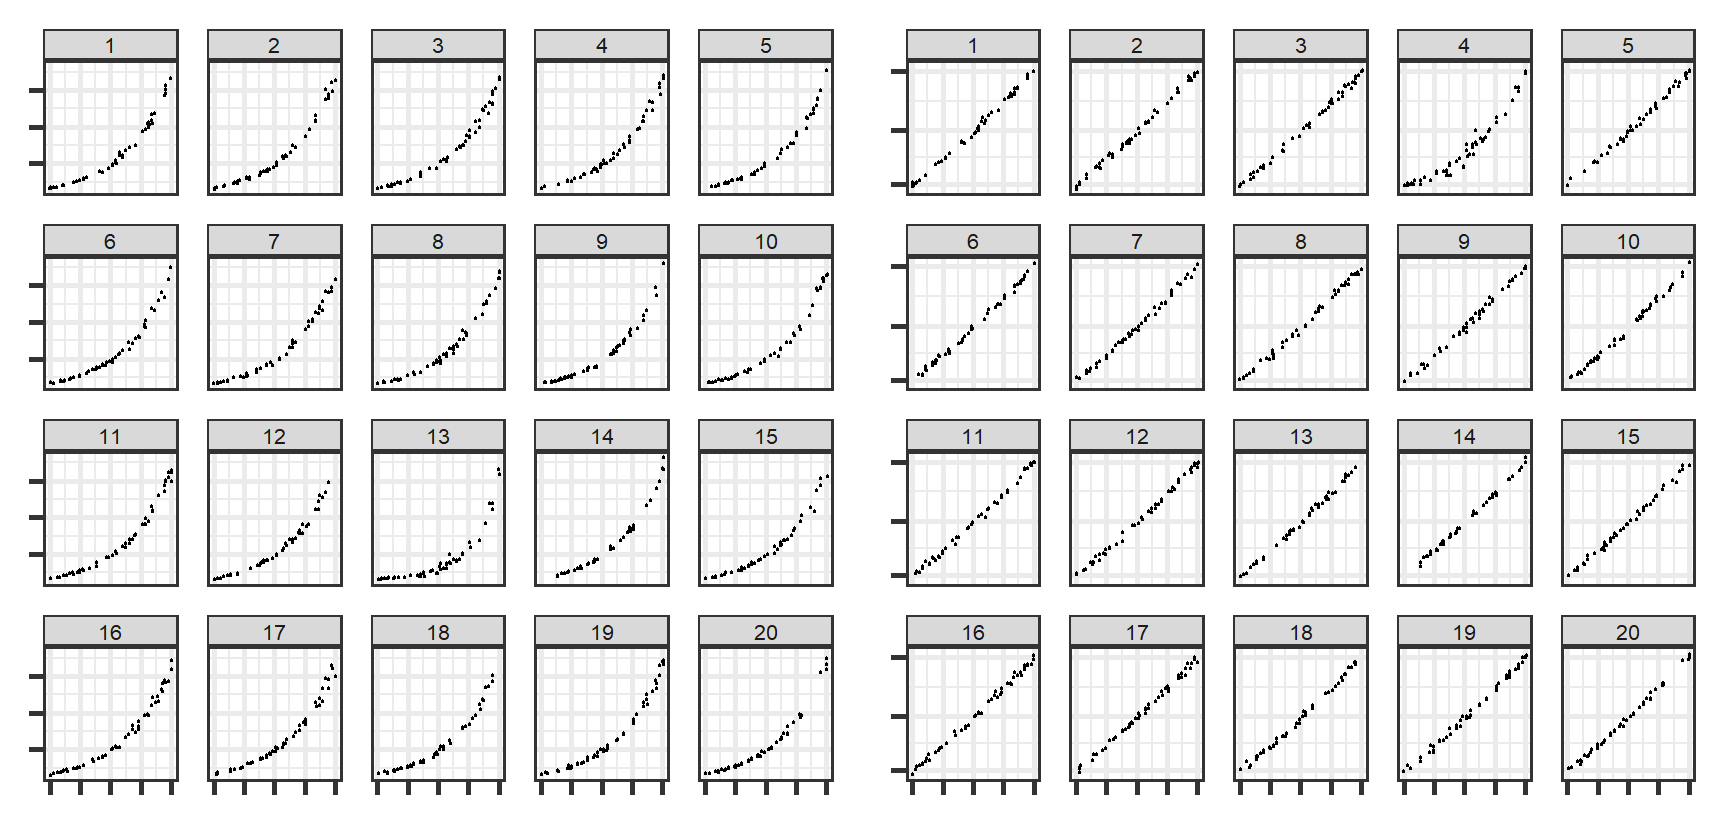
\includegraphics[width=\linewidth]{thesis_files/figure-latex/lineup-example-1} 

}

\caption{Lineup example}\label{fig:lineup-example}
\end{figure}

\hypertarget{data-generation}{%
\section{Data Generation}\label{data-generation}}

In this study, both the target and null data sets were generated by simulating data from an exponential model; the models differ in the parameters selected for the null and target panels.
In order to guarantee the simulated data spans the same domain and range of values, we implemented a domain constraint of \(x\in [0,20]\) and a range constraint of \(y\in [10,100]\) with \(N = 50\) points randomly assigned throughout the domain and mapped to the y-axis using the exponential model with the selected parameters.
These constraints provide some assurance that participants who select the target plot are doing so because of their visual perception differentiating between curvature or growth rate rather than different starting or ending values.

We simulated data based on a three-parameter exponential model with multiplicative errors:

\begin{align}
y_i & = \alpha\cdot e^{\beta\cdot x_i + \epsilon_i} + \theta \\
\text{with } \epsilon_i & \sim N(0, \sigma^2). \nonumber
\end{align}

\noindent The parameters \(\alpha\) and \(\theta\) are adjusted based on \(\beta\) and \(\sigma^2\) to guarantee the range and domain constraints are met.
The model generated \(N = 50\) points \((x_i, y_i), i = 1,...,N\) where \(x\) and \(y\) have an increasing exponential relationship.
The heuristic data generation procedure is described below:

\textit{Algorithm 2.1.1: Paremeter Estimation}

Input Parameters: domain \(x\in[0,20]\), range \(y\in[10,100]\), midpoint \(x_{mid}\).

Output: estimated model parameters \(\hat\alpha, \hat\beta, \hat\theta\)

\begin{enumerate}
\def\labelenumi{\arabic{enumi}.}
\item
  Determine the \(y=-x\) line scaled to fit the assigned domain and range.
\item
  Map the values \(x_{mid} - 0.1\) and \(x_{mid} + 0.1\) to the \(y=-x\) line for two additional points.
\item
  From the set points \((x_k, y_k)\) for \(k = 1,2,3,4\), obtain the coefficients from the linear model \(\ln(y_k) = b_0 +b_1x_k\) to obtain starting values - \(\alpha_0 = e^{b_0}, \beta_0 = b_1, \theta_0 = 0.5\cdot \min(y)\)
\item
  Using the \texttt{nls()} function from the \texttt{stats} package in Rstudio and the starting parameter values - \(\alpha_0, \beta_0, \theta_0\) - fit the nonlinear model, \(y_k = \alpha\cdot e^{\beta\cdot x_k}+\theta\) to obtain estimated parameter values - \(\hat\alpha, \hat\beta, \hat\theta.\)
\end{enumerate}

\noindent\textit{Algorithm 2.1.2: Exponential Simulation}

Input Paremeters: sample size \(N = 50\), estimated parameters \(\hat\alpha\), \(\hat\beta\), and \(\hat\theta\), \(\sigma\) standard deviation from the exponential curve.

Output Parameters: \(N\) points, in the form of vectors \(\mathbf{x}\) and \(\mathbf{y}\).

\begin{enumerate}
\def\labelenumi{\arabic{enumi}.}
\item
  Generate \(\tilde x_j, j = 1,..., N\cdot \frac{3}{4}\) as a sequence of evenly spaced points in \([0,20]\). This ensures the full domain of \(x\) is used, fulfilling the constraints of spanning the same domain and range for each parameter combination.
\item
  Obtain \(\tilde x_i, i = 1,...N\) by sampling \(N = 50\) values from the set of \(\tilde x_j\) values. This gaurantees some variability and potential clustring in the exponential growth curve disrupting the perception due to continuity of points.
\item
  Obtain the final \(x_i\) values by jittering \(\tilde x_i\).
\item
  Calculate \(\tilde\alpha = \frac{\hat\alpha}{e^{\sigma^2/2}}.\) This ensures that the range of simulated values for different standard devaition parameters has an equal expected value for a given rate of change due to the non-constant variance across the domain.
\item
  Generate \(y_i = \tilde\alpha\cdot e^{\hat\beta x_i + e_i}+\hat\theta\) where \(e_i\sim N(0,\sigma^2).\)
\end{enumerate}

\hypertarget{parameter-selection}{%
\section{Parameter Selection}\label{parameter-selection}}

For each level of difficulty, we simulated 1000 data sets of \((x_{ij}, y_{ij})\) points for \(i = 1,...,50\) and \(j = 1...10\).
Each generated \(x_i\) point from \textit{Algorithm 2.1.2} was replicated 10 times. Then the lack of fit statistic (LOF) was computed for each simulated data set by calculating the deviation of the data from a linear line.
Plotting the density curves of the LOF statistics for each level of difficulty choice allows us to evaluate the ability of differentiating between the difficulty levels and thus detecting the target plot.
In Figure \ref{fig:lof-density-curves}, we can see the densities of each of the three difficulty levels.
While the LOF statistic provides us a numerical value for discriminating between the difficulty levels, we cannot directly relate this to the perceptual discriminability; it serves primarily as an approximation to ensure that we are testing parameters at several distinct levels of difficulty.

\begin{figure}

{\centering 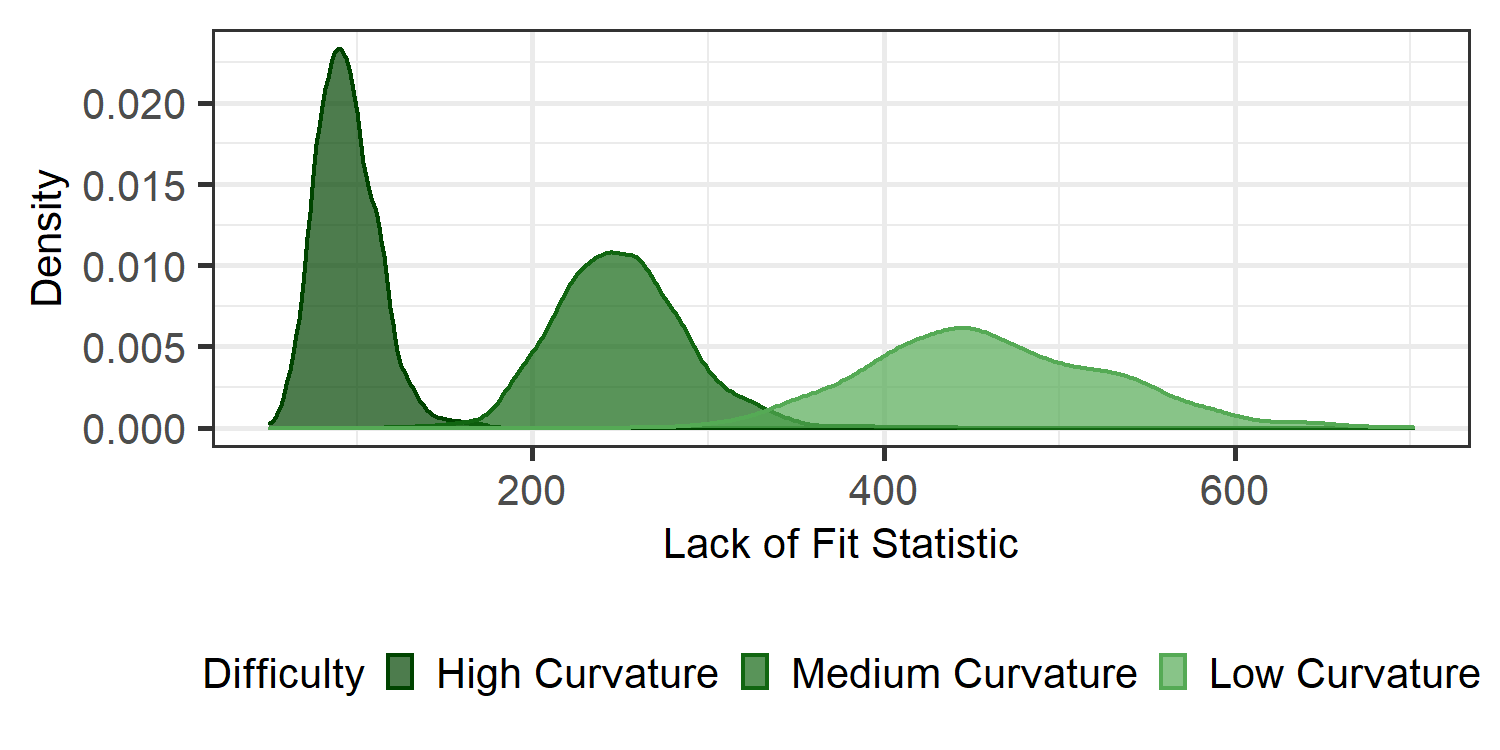
\includegraphics[width=\linewidth]{thesis_files/figure-latex/lof-density-curves-1} 

}

\caption{Lack of fit statistic density curves}\label{fig:lof-density-curves}
\end{figure}

Final parameter estimates are shown in Table \ref{tab:parameter-data}.

\begin{table}

\caption{\label{tab:parameter-data}Lineup data simulation final parameters}
\centering
\begin{tabular}[t]{ccccccc}
\toprule
 & $x_{mid}$ & $\hat\alpha$ & $\tilde\alpha$ & $\hat\beta$ & $\hat\theta$ & $\hat\sigma$\\
\midrule
Easy & 14.5 & 0.91 & 0.88 & 0.23 & 9.10 & 0.25\\
Medium & 13.0 & 6.86 & 6.82 & 0.13 & 3.14 & 0.12\\
Hard & 11.5 & 37.26 & 37.22 & 0.06 & -27.26 & 0.05\\
\bottomrule
\end{tabular}
\end{table}

\hypertarget{lineup-setup}{%
\section{Lineup Setup}\label{lineup-setup}}

Lineup plots were generated by mapping one simulated data set corresponding to difficulty level A to a scatter plot to be identified as the target plot while multiple simulated data sets corresponding to difficulty level B were individually mapped to scatter plots for the null plots.
For example, a target plot with simulated data following an increasing exponential curve with obvious curvature is embedded within null plots with simulated data following an increasing exponential trend that is almost linear (i.e.~Hard Null - Easy Target).
By our constraints, the target plot and null plots will span a similar domain and range.
There are a total of six (i.e.~\(3!\cdot 2!\)) lineup parameter combinations.
Two sets of each lineup parameter combination were simulated (total of 12 test data sets) and plotted on both the linear scale and the log scale (total of 24 test lineup plots).
In addition, there are three parameter combinations which generate homogeneous ``Rorschach'' lineups, where all panels are from the same distribution. Each participant evaluated one of these lineups, but for simplicity, these evaluations are not described in this paper.

\hypertarget{study-design}{%
\section{Study Design}\label{study-design}}

Each participant was shown a total of thirteen lineup plots (twelve test lineup plots and one Rorschach lineup plot). Participants were randomly assigned one of the two replicate data sets for each of the six unique lineup parameter combinations. For each assigned test data set, the participant was shown the lineup plot corresponding to both the linear scale and the log scale. For the additional Rorschach lineup plot, participants were randomly assigned one data set shown on either the linear or the log scale. The order of the thirteen lineup plots shown was randomized for each participant.

Participants above the age of majority were recruited from Reddit's Visualization and Sample Size communities.
Since participants recruited on Reddit were not compensated for their time, most participants have an interest in data visualization research.
Previous literature suggests that prior mathematical knowledge or experience with exponential data is not associated with the outcome of graphical experiments (\textbf{vanderplasSpatialReasoningData2016?}).
Participants completed the experiment using a Shiny applet (\url{https://shiny.srvanderplas.com/log-study/}).

Participants were shown a series of lineup plots and asked to identify the plot that was most different from the others.
On each plot, participants were asked to justify their choice and provide their level of confidence in their choice.
The goal of this experimental task is to test an individuals ability to perceptually differentiate exponentially increasing trends with differing levels of curvature on both the linear and log scale.

\hypertarget{results}{%
\section{Results}\label{results}}

Participant recruitment through Reddit occurred over the course of two weeks during which 58 individuals completed 518 unique test lineup evaluations. Previous studies have found that results do not differ on lineup-related tasks between Reddit and e.g.~Amazon Mechanical Turk (VanderPlas \& Hofmann, 2017).
Participants who completed fewer than 6 lineup evaluations were removed from the study (17 participants, 41 evaluations).
The final data set included a total of 41 participants and 477 lineup evaluations.
Each plot was evaluated by between 18 and 28 individuals (Mean: 21.77, SD: 2.29).
In 67\% of the 477 lineup evaluations, participants correctly identified the target panel.

Target plot identification was analyzed using the Glimmix Procedure in SAS 9.4.
Each lineup plot evaluated was assigned a value based on the participant response (correct = 1, not correct = 0).
The binary response was analyzed using a generalized linear mixed model following a binomial distribution with a logit link function following a row-column blocking design to account for the variation due to participant and data set respectively. See model details and estimates in \ear{Appendix Reference}.

On both the log and linear scales, the highest accuracy occurred in lineup plots where the target model and null model had large curvature differences (Easy Null - Hard Target; Hard Null - Easy Target).
There is a decrease in accuracy on the linear scale when comparing a target plot with less curvature to null plots with more curvature (Easy Null - Medium Target; Medium Null - Hard Target).
Best, Smith, \& Stubbs (2007) found that accuracy of identifying the correct curve type was higher when nonlinear trends were presented indicating that it is hard to say something is linear (i.e.~something has less curvature), but easy to say that it is not linear; our results concur with this observation.
Overall, there are no significant differences in accuracy between curvature combinations when data is presented on a log scale indicating participants were consistent in their success of identifying the target panel on the log scale.
Figure \ref{fig:odds-ratio-plot} displays the estimated (log) odds ratio of successfully identifying the target panel on the log scale compared to the linear scale.
The choice of scale has no impact if curvature differences are large (Hard Null - Easy Target; Easy Null - Hard Target).
However, presenting data on the log scale makes us more sensitive to slight changes in curvature (Medium Null - Easy Target; Medium Null - Hard Target; Easy Null - Medium Target).
An exception occurs when identifying a plot with curvature embedded in null plots close to a linear trend (Hard Null - Medium Target), again supporting the claim that it is easy to identify a curve in a bunch of lines but much harder to identify a line in a bunch of curves (Best, Smith, \& Stubbs, 2007).

\begin{figure}

{\centering 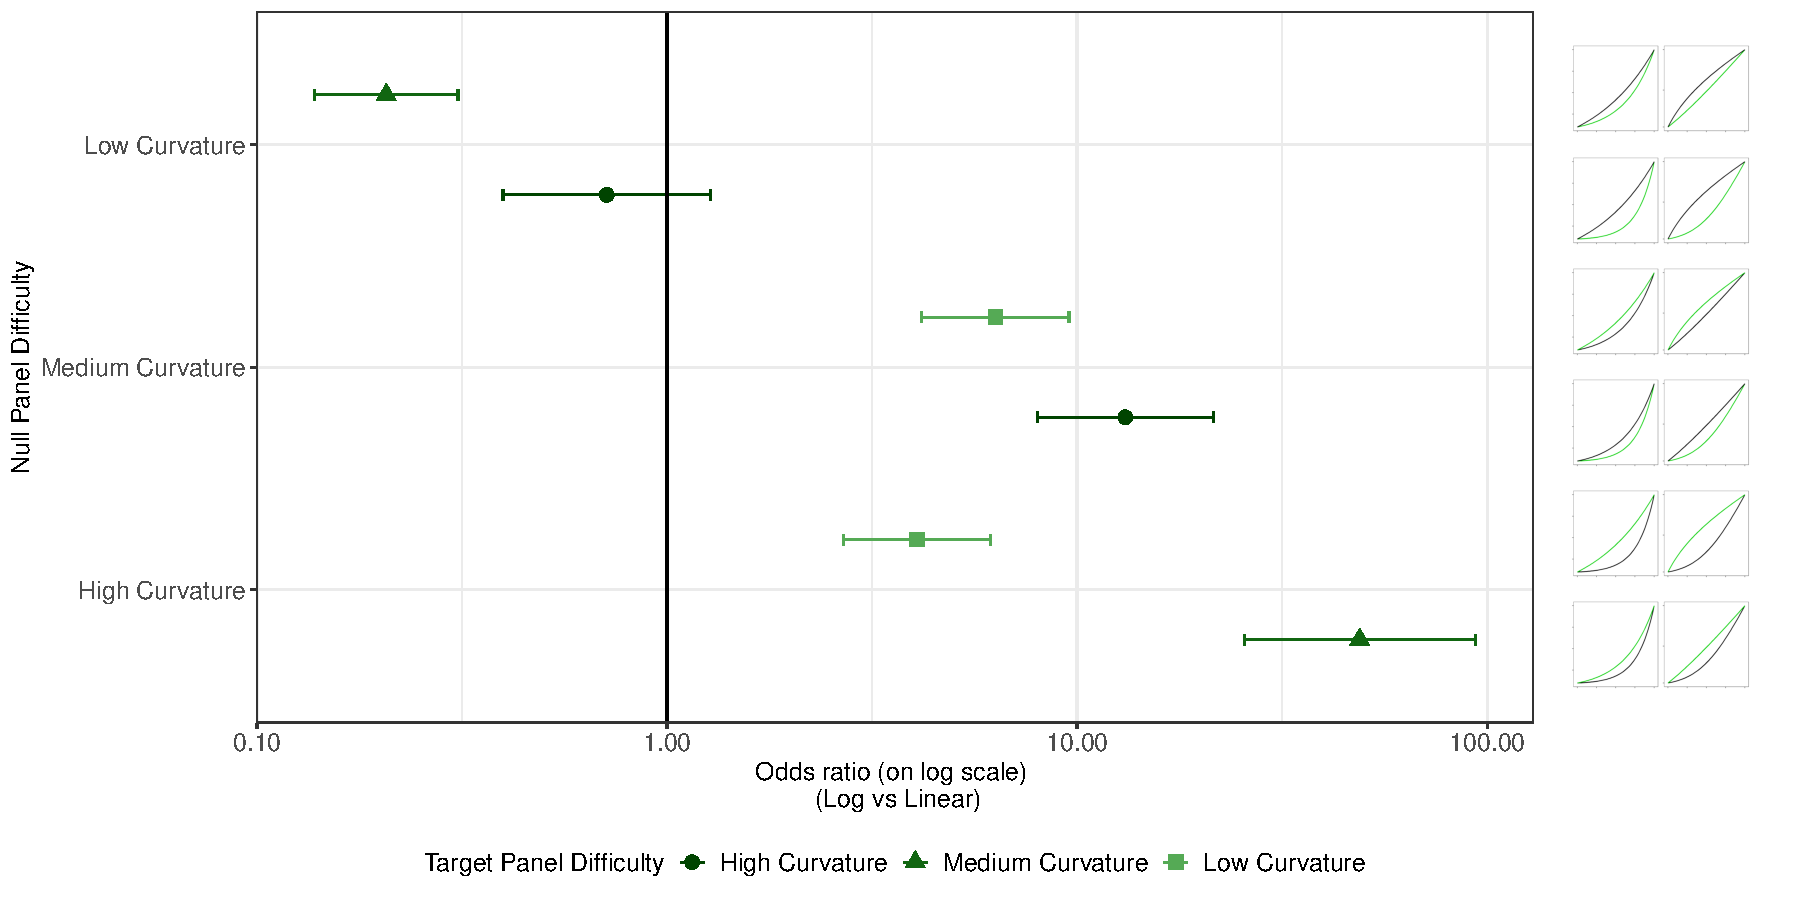
\includegraphics[width=\linewidth]{thesis_files/figure-latex/odds-ratio-plot-1} 

}

\caption{Lineups log(odds) results}\label{fig:odds-ratio-plot}
\end{figure}

\hypertarget{discussion-and-conclusion}{%
\section{Discussion and Conclusion}\label{discussion-and-conclusion}}

The overall goal of this paper is to provide basic research to support the principles used to guide design decisions in scientific visualizations of exponential data.
In this study, we explore the use of linear and log scales to determine whether our ability to notice differences in exponentially increasing trends is impacted by the choice of scale.
Our results indicated that when there was a large difference in curvature between the target plot and null plots, the choice of scale had no impact and participants accurately differentiated between the two curves on both the linear and log scale.
However, displaying exponentially increasing data on a log scale improved the accuracy of differentiating between models with slight curvature differences.
An exception occurred when identifying a plot with curvature embedded in surrounding plots closely relating to a linear trend, indicating that it is easy to identify a curve in a group of lines but much harder to identify a line in a group of curves.
The use of visual inference to identify these guidelines suggests that there are \emph{perceptual} advantages to log scales when differences are subtle.
What remains to be seen is whether there are cognitive disadvantages to log scales: do log scales make it harder to make use of graphical information?

\hypertarget{youdrawit}{%
\chapter{Prediction with you draw it}\label{youdrawit}}

\hypertarget{introduction-1}{%
\section{Introduction}\label{introduction-1}}

\hypertarget{estimation}{%
\chapter{Numerical Translation and Estimation}\label{estimation}}

\hypertarget{conclusion}{%
\chapter{Conclusion}\label{conclusion}}

\appendix

\hypertarget{the-first-appendix}{%
\chapter{The First Appendix}\label{the-first-appendix}}

\hypertarget{the-second-appendix}{%
\chapter{The Second Appendix}\label{the-second-appendix}}

\backmatter

\hypertarget{references}{%
\chapter*{References}\label{references}}
\addcontentsline{toc}{chapter}{References}

\noindent

\setlength{\parindent}{-0.20in}
\setlength{\leftskip}{0.20in}
\setlength{\parskip}{8pt}

\hypertarget{refs}{}
\begin{CSLReferences}{1}{0}
\leavevmode\hypertarget{ref-noauthor_interactive_nodate}{}%
An interactive visualization of {COVID}-19 {{}} 91-{DIVOC}. (n.d.). Retrieved from \url{https://91-divoc.com/pages/covid-visualization/}

\leavevmode\hypertarget{ref-bavel_using_2020}{}%
Bavel, J. J. V., Baicker, K., Boggio, P. S., Capraro, V., Cichocka, A., Cikara, M., \ldots{} Willer, R. (2020). Using social and behavioural science to support {COVID}-19 pandemic response. \emph{Nature Human Behaviour}, \emph{4}(5), 460--471. http://doi.org/\href{https://doi.org/10.1038/s41562-020-0884-z}{10.1038/s41562-020-0884-z}

\leavevmode\hypertarget{ref-best_perception_2007}{}%
Best, L. A., Smith, L. D., \& Stubbs, D. A. (2007). Perception of {Linear} and {Nonlinear} {Trends}: {Using} {Slope} and {Curvature} {Information} to {Make} {Trend} {Discriminations}. \emph{Perceptual and Motor Skills}, \emph{104}(3), 707--721. http://doi.org/\href{https://doi.org/10.2466/pms.104.3.707-721}{10.2466/pms.104.3.707-721}

\leavevmode\hypertarget{ref-buja_statistical_2009}{}%
Buja, A., Cook, D., Hofmann, H., Lawrence, M., Lee, E.-K., Swayne, D. F., \& Wickham, H. (2009). Statistical inference for exploratory data analysis and model diagnostics. \emph{Philosophical Transactions of the Royal Society A: Mathematical, Physical and Engineering Sciences}, \emph{367}(1906), 4361--4383. http://doi.org/\href{https://doi.org/10.1098/rsta.2009.0120}{10.1098/rsta.2009.0120}

\leavevmode\hypertarget{ref-cleveland_graphical_1984}{}%
Cleveland, W. S., \& McGill, R. (1984). Graphical {Perception}: {Theory}, {Experimentation}, and {Application} to the {Development} of {Graphical} {Methods}. Retrieved from \url{http://euclid.psych.yorku.ca/www/psy6135/papers/ClevelandMcGill1984.pdf}

\leavevmode\hypertarget{ref-cleveland_graphical_1985}{}%
Cleveland, W. S., \& McGill, R. (1985). Graphical {Perception} and {Graphical} {Methods} for {Analyzing} {Scientific} {Data}. \emph{Science, New Series}, \emph{229}(4716), 828--833. Retrieved from \url{http://www.jstor.org/stable/1695272}

\leavevmode\hypertarget{ref-noauthor_coronavirus_nodate}{}%
Coronavirus chart: See how your country compares {{}} {Free} to read {{}} {Financial} {Times}. (n.d.). Retrieved from \url{https://ig.ft.com/coronavirus-chart/?areas=eur}

\leavevmode\hypertarget{ref-gmbh_youve_2020}{}%
GmbH, D. (2020, July). You've informed the public with visualizations about the coronavirus. {Thank} you. \emph{Chartable}. Retrieved from \url{https://blog.datawrapper.de/datawrapper-effect-corona/index.html}

\leavevmode\hypertarget{ref-gordon_statistician_2015}{}%
Gordon, I., \& Finch, S. (2015). Statistician {Heal} {Thyself}: {Have} {We} {Lost} the {Plot}? \emph{Journal of Computational and Graphical Statistics}, \emph{24}(4), 1210--1229. http://doi.org/\href{https://doi.org/10.1080/10618600.2014.989324}{10.1080/10618600.2014.989324}

\leavevmode\hypertarget{ref-haemer_presentation_1949}{}%
Haemer, K. W., \& Kelley, T. L. (1949). Presentation {Problems}: {Suiting} the {Chart} to the {Audience}: {Common} {Graphic} {Devices} {Classified} {According} to {Ease} of {Reading}. \emph{The American Statistician}, \emph{3}(5), 11--11. http://doi.org/\href{https://doi.org/10.1080/00031305.1949.10501608}{10.1080/00031305.1949.10501608}

\leavevmode\hypertarget{ref-heckler_student_2013}{}%
Heckler, A. F., Mikula, B., \& Rosenblatt, R. (2013). Student accuracy in reading logarithmic plots: {The} problem and how to fix it. In \emph{2013 {IEEE} {Frontiers} in {Education} {Conference} ({FIE})} (pp. 1066--1071). http://doi.org/\href{https://doi.org/10.1109/FIE.2013.6684990}{10.1109/FIE.2013.6684990}

\leavevmode\hypertarget{ref-jones_polynomial_1977}{}%
Jones, G. V. (1977). Polynomial perception of exponential growth. \emph{Perception \& Psychophysics}, \emph{21}(2), 197--198. http://doi.org/\href{https://doi.org/10.3758/BF03198726}{10.3758/BF03198726}

\leavevmode\hypertarget{ref-lewandowsky_perception_1989}{}%
Lewandowsky, S., \& Spence, I. (1989). The {Perception} of {Statistical} {Graphs}. \emph{Sociological Methods \& Research}, \emph{18}(2-3), 200--242. http://doi.org/\href{https://doi.org/10.1177/0049124189018002002}{10.1177/0049124189018002002}

\leavevmode\hypertarget{ref-noauthor_log_nodate}{}%
Log or {Linear}? {Distinct} {Intuitions} of the {Number} {Scale} in {Western} and {Amazonian} {Indigene} {Cultures}. (n.d.), 5.

\leavevmode\hypertarget{ref-noauthor_log_nodate-1}{}%
Log {Scale}. (n.d.). \emph{xkcd}. Retrieved from \url{https://xkcd.com/1162/}

\leavevmode\hypertarget{ref-mackinnon_feedback_1991}{}%
Mackinnon, A. J., \& Wearing, A. J. (1991). Feedback and the forecasting of exponential change. \emph{Acta Psychologica}, \emph{76}(2), 177--191. http://doi.org/\href{https://doi.org/10.1016/0001-6918(91)90045-2}{10.1016/0001-6918(91)90045-2}

\leavevmode\hypertarget{ref-majumder_validation_2013}{}%
Majumder, M., Hofmann, H., \& Cook, D. (2013). Validation of {Visual} {Statistical} {Inference}, {Applied} to {Linear} {Models}. \emph{Journal of the American Statistical Association}, \emph{108}(503), 942--956. http://doi.org/\href{https://doi.org/10.1080/01621459.2013.808157}{10.1080/01621459.2013.808157}

\leavevmode\hypertarget{ref-menge_logarithmic_2018}{}%
Menge, D. N. L., MacPherson, A. C., Bytnerowicz, T. A., Quebbeman, A. W., Schwartz, N. B., Taylor, B. N., \& Wolf, A. A. (2018). Logarithmic scales in ecological data presentation may cause misinterpretation. \emph{Nature Ecology \& Evolution}, \emph{2}(9), 1393--1402. http://doi.org/\href{https://doi.org/10.1038/s41559-018-0610-7}{10.1038/s41559-018-0610-7}

\leavevmode\hypertarget{ref-nieder_coding_nodate}{}%
Nieder, A., \& Miller, E. K. (n.d.). Coding of {Cognitive} {Magnitude}: {Compressed} {Scaling} of {Numerical} {Information} in the {Primate} {Prefrontal} {Cortex}, 9.

\leavevmode\hypertarget{ref-romano_scale_2020}{}%
Romano, A., Sotis, C., Dominioni, G., \& Guidi, S. (2020). \emph{The {Scale} of {COVID}-19 {Graphs} {Affects} {Understanding}, {Attitudes}, and {Policy} {Preferences}} (\{SSRN\} \{Scholarly\} \{Paper\} No. ID 3588511). Rochester, NY: Social Science Research Network. Retrieved from \url{https://papers.ssrn.com/abstract=3588511}

\leavevmode\hypertarget{ref-shah_graphs_nodate}{}%
Shah, P., Mayer, R. E., \& Hegarty, M. (n.d.). Graphs as {Aids} to {Knowledge} {Construction}: {Signaling} {Techniques} for {Guiding} the {Process} of {Graph} {Comprehension}, 13.

\leavevmode\hypertarget{ref-siegler_numerical_2017}{}%
Siegler, R. S., \& Braithwaite, D. W. (2017). Numerical {Development}. \emph{Annual Review of Psychology}, \emph{68}(1), 187--213. http://doi.org/\href{https://doi.org/10.1146/annurev-psych-010416-044101}{10.1146/annurev-psych-010416-044101}

\leavevmode\hypertarget{ref-sun_framework_2012}{}%
Sun, J. Z., Wang, G. I., Goyal, V. K., \& Varshney, L. R. (2012). A framework for {Bayesian} optimality of psychophysical laws. \emph{Journal of Mathematical Psychology}, \emph{56}(6), 495--501. http://doi.org/\href{https://doi.org/10.1016/j.jmp.2012.08.002}{10.1016/j.jmp.2012.08.002}

\leavevmode\hypertarget{ref-unwin_why_2020}{}%
Unwin, A. (2020). Why is {Data} {Visualization} {Important}? {What} is {Important} in {Data} {Visualization}? \emph{Harvard Data Science Review}. http://doi.org/\href{https://doi.org/10.1162/99608f92.8ae4d525}{10.1162/99608f92.8ae4d525}

\leavevmode\hypertarget{ref-uri_presentation_1948}{}%
Uri, G., \& Haemer, K. (1948). Presentation {Problems}: {Graphic} {Representation} for {Multiple} {Linear} {Correlation}. \emph{The American Statistician}, \emph{2}(6), 19--19. http://doi.org/\href{https://doi.org/10.1080/00031305.1948.10483416}{10.1080/00031305.1948.10483416}

\leavevmode\hypertarget{ref-vanderplas_testing_2020}{}%
Vanderplas, S., Cook, D., \& Hofmann, H. (2020). Testing {Statistical} {Charts}: {What} {Makes} a {Good} {Graph}? \emph{Annual Review of Statistics and Its Application}, \emph{7}(1), 61--88. http://doi.org/\href{https://doi.org/10.1146/annurev-statistics-031219-041252}{10.1146/annurev-statistics-031219-041252}

\leavevmode\hypertarget{ref-vanderplas_clusters_2017}{}%
VanderPlas, S., \& Hofmann, H. (2017). Clusters {Beat} {Trend}!? {Testing} {Feature} {Hierarchy} in {Statistical} {Graphics}. \emph{Journal of Computational and Graphical Statistics}, \emph{26}(2), 231--242. http://doi.org/\href{https://doi.org/10.1080/10618600.2016.1209116}{10.1080/10618600.2016.1209116}

\leavevmode\hypertarget{ref-wagenaar_misperception_1975}{}%
Wagenaar, W. A., \& Sagaria, S. D. (1975). Misperception of exponential growth. \emph{Perception \& Psychophysics}, \emph{18}(6), 416--422. http://doi.org/\href{https://doi.org/10.3758/BF03204114}{10.3758/BF03204114}

\leavevmode\hypertarget{ref-wickham2016r}{}%
Wickham, H., \& Grolemund, G. (2016). \emph{R for data science: Import, tidy, transform, visualize, and model data}. " O'Reilly Media, Inc.".

\end{CSLReferences}


%% backmatter is needed at the end of the main body of your thesis to
%% set up page numbering correctly for the remainder of the thesis
\backmatter

%% Start the correct formatting for the appendices
% \appendix
%% Input each appendix here
% \input{./appendix_a}

%% Bibliography goes here (You better have one)
%% BibTeX is your friend

% \bibliographystyle{alpha}  % or use  abbrv to abbreviate first names and use numerical indices
\bibliographystyle{abbrv}  % or use  abbrv to abbreviate first names and use numerical indices
%% Add your BibTex file here (don't include the .bib)
\bibliography{./references}



%% Index go here (if you have one)
\end{document}
